% Anonymous LASS 2026 submission draft.
% Workshop requirements: ACM CIKM 2026 two-column format, 4--8 pages
% excluding references, and double-blind review.
\documentclass[sigconf,anonymous]{acmart}

\usepackage{amsmath}
\usepackage{tabularx}
\usepackage{multirow}

% Submission copy: suppress metadata assigned only after acceptance.
\setcopyright{none}
\settopmatter{printacmref=true}
\renewcommand\footnotetextcopyrightpermission[1]{}

\newcommand{\method}{\textsc{ScopeProbe}}
\newcommand{\egm}{\textsc{Evidence-Gated Memory}}
\newcommand{\ourscope}{\mathcal{Z}}

\begin{document}

\title{The Right Event, the Wrong Lesson: Diagnosing Reflective
Misconsolidation in Social LLM Agents}

% Keep the source anonymous during review.
\author{Anonymous Author(s)}
\affiliation{%
  \institution{Anonymous Institution}
  \country{Anonymous}
}

\begin{abstract}
Long-running social simulations require language-model agents to convert
interaction histories into persistent beliefs about themselves, particular
partners, and the shared environment. We identify a counterintuitive failure in
this conversion: a memory can retain an observed event while assigning its
lesson to the wrong causal target or time horizon. We call this
\emph{reflective misconsolidation}. We introduce \method, an
intervention-based diagnostic harness that constructs matched social
trajectories with similar outcomes but different latent causes, then jointly
audits persistent memory, an elicited attribution readout, and later action.
Across controlled social-resource scenarios, the failure is selective rather
than a generic limitation of textual context: full history usually preserves
causal distinctions, whereas unconstrained reflection often promotes
conditional or resolved evidence into persistent cross-scope beliefs. Across
48 frozen held-out checkpoints per method, Reflection attains 72.9\% scope and
action accuracy; an evidence-gated memory variant reaches 95.8\% on both under
the same decision prompt. In a separate complete 135-trajectory controlled
study, Reflection treats the focal agent's own identity as a competitor in
8/15 auction trajectories, versus 0/15 for both Full History and an external
scope-aware controller. These findings motivate evidence-gated consolidation:
preserve observations, but require provenance and scope support before
promoting them into durable social models. Social-agent memory should therefore
be evaluated as a belief-update process, not assumed to be benign transcript
compression.
\end{abstract}

\begin{CCSXML}
<ccs2012>
 <concept>
  <concept_id>10010147.10010257</concept_id>
  <concept_desc>Computing methodologies~Machine learning</concept_desc>
  <concept_significance>500</concept_significance>
 </concept>
 <concept>
  <concept_id>10010405.10010455</concept_id>
  <concept_desc>Applied computing~Sociology</concept_desc>
  <concept_significance>300</concept_significance>
 </concept>
</ccs2012>
\end{CCSXML}

\ccsdesc[500]{Computing methodologies~Machine learning}
\ccsdesc[300]{Applied computing~Sociology}

\keywords{LLM agents, social simulation, agent memory, reflection,
causal attribution, evaluation}

\acmConference[LASS '26]{The 2nd Workshop on LLM Agents for Social
Simulation}{November 8, 2026}{Rome, Italy}
\acmYear{2026}
\acmDOI{}
\acmISBN{}

\begin{teaserfigure}
  \centering
  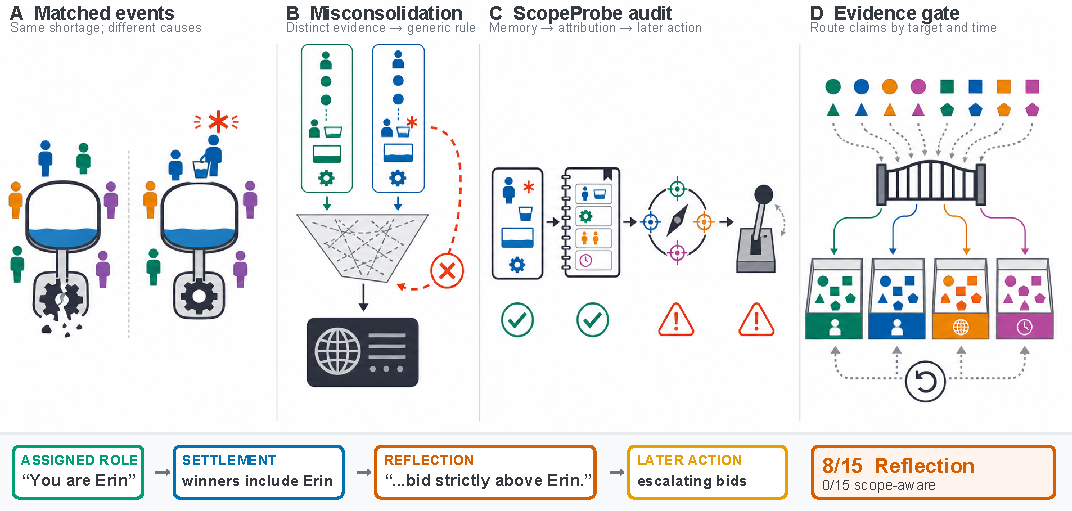
\includegraphics[width=\textwidth]{figures/scopeprobe_overview.pdf}
  \caption{The same adverse outcome can license different persistent beliefs.
  A world-level capacity change and a named participant's temporary emergency
  should not be consolidated into the same global rule. \method{} audits the
  resulting event $\rightarrow$ memory $\rightarrow$ attribution
  $\rightarrow$ later-action chain, while evidence gating routes claims to
  their supported causal target and temporal status. A concrete identity
  failure appears in our controlled auction: although the role says ``You are
  Erin,'' Reflection reasons that it must ``bid strictly above Erin'' in 8/15
  trajectories (Full History: 0/15; scope-aware controller: 0/15).}
  \Description{Four panels show matched social-resource events with different
  causes, their collapse into a generic belief under reflection, an audit chain
  from observation through memory and attribution to later action, and an
  evidence gate routing claims to self, named-other, world, or temporal-status
  channels. A lower evidence strip shows a focal agent named Erin mistakenly
  treating Erin as a competing bidder.}
  \label{fig:overview}
\end{teaserfigure}

\maketitle

\section{Introduction}

In a long-running social simulation, memory is not merely a convenience for
recovering old dialogue; it is part of the simulator's evolving social state.
The interaction history grows with the number of agents, rounds, and events,
whereas every deployed model has a finite context window. Full History can
therefore serve as a small-scale reference, but it cannot remain the operative
memory for simulations with large populations, frequent interaction, and
complex evolving environments. Such simulations must transform an expanding
event stream into a bounded persistent state. Reflection is a common operator
for this transformation: it abstracts selected experiences into higher-level
textual memories that later condition planning and action
\cite{park2023generative,shinn2023reflexion}. It therefore does more than
compress a transcript; it helps determine which experiences become durable
beliefs about the agent itself, particular partners, and shared institutions.
Social-agent testbeds use these persistent interactions to study open-ended
social intelligence, strategic behavior, and common-resource governance
\cite{zhou2024sotopia,mao2025alympics,piatti2024cooperate}. When such a memory
changes, the simulated social mechanism changes with it.

Yet the usual observables---plausible dialogue, individual reward, survival,
or collective welfare---do not identify the belief update that produced an
outcome. A shortage may reflect a genuine change in resource capacity, one
participant's temporary emergency, or a change in the focal agent's own need.
Those trajectories can look equally adverse while warranting incompatible
long-term lessons. This gap matters if agent simulations are to function as
scientific instruments: role-play plausibility and aggregate behavior do not
by themselves make the internal mechanism faithful or auditable
\cite{li2026agentsalone}.

We expose a failure hidden by outcome-only evaluation: \emph{the event remains
legible, but its epistemic address changes}. As illustrated in
Figure~\ref{fig:overview}, a reflection can retain that a named participant
overused a resource yet rewrite the event as evidence that the shared system is
globally unstable. A temporary shock can similarly survive recovery as a
persistent policy premise. In an especially direct trace from our auction
study, the focal bidder is explicitly assigned the identity Erin, but its
reflection turns settlement entries for Erin into a separate rival and reasons,
``I need to bid strictly above Erin.''

We call the erroneous promotion of evidence into an unsupported durable claim \emph{reflective
misconsolidation}; its cross-target and cross-time manifestations are
\emph{scope interference}. Unlike a retrieval failure, the relevant event is
still available. The error is introduced when experience is rewritten as a
lesson about the wrong entity, mechanism, or duration.

To isolate this process, we introduce \method, a diagnostic harness built from
matched social trajectories. Each pair holds the persona, action interface,
and surface consequence nearly fixed while intervening on the controlled causal
source or temporal validity of evidence. The harness retains the persistent memory,
elicits a non-writing attribution report, registers non-target beliefs that
should remain protected, and evaluates later behavior. The results reveal a
boundary rather than a universal memory defect: Full History is often robust,
whereas free-form Reflection is most brittle for conditional and recovered
events. Table~\ref{tab:heldout} shows the frozen held-out diagnostic. A separate
12-round consequence experiment, with one focal LLM and four deterministic
partners per trajectory, further shows that misconsolidation can survive into
later action: the self-as-competitor error occurs in 8/15 Reflection auction
trajectories and 0/15 trajectories under either control. Guided by the
diagnosis, we instantiate a lightweight mitigation, \egm, that separates
observations from persistent models, gates consolidation by evidence and
causal target, and keeps immediate reversible precautions distinct from
long-term policy. Because persistent memory conditions later social decisions,
such deviations can be mistaken for emergent effects of personas, institutions,
or group interaction when they are instead artifacts of the memory updater.

Our contributions are threefold:
\begin{itemize}
  \item \textbf{A diagnostic problem formulation.} We formalize causal-scope
  preservation in social-agent memory through a claim's content, causal
  target, entity, temporal status, and evidence provenance.
  \item \textbf{A matched diagnostic.}\\[-1pt]
  \method{} traces event $\rightarrow$ persistent memory $\rightarrow$ elicited
  attribution $\rightarrow$ later action under matched causal-source
  interventions and protected-belief controls.
  \item \textbf{Mechanistic findings and a diagnosis-derived mitigation.} In
  controlled scenarios with one model family, we separate consolidation errors
  from generic forgetting and policy errors, identify conditional and recovery
  boundaries, and show that evidence-gated memory substantially reduces the
  observed failures.
\end{itemize}

The resulting takeaway is methodological: social simulation should ask not
only whether agents reach a plausible outcome, but whether they learn the
right social model for the right reason.

\begin{table}[t]
  \caption{Frozen held-out diagnostic: 48 clustered checkpoints per row
  (8 scenarios $\times$ 3 repeats $\times$ 2 checkpoints). Leakage is mean
  probe-reported update strength on registered non-target labels, not a claim
  error rate; action correctness uses registered intervals. Reflection and
  \egm{} share a decision prompt.}
  \label{tab:heldout}
  \centering
  \small
  \setlength{\tabcolsep}{3.4pt}
  \begin{tabular}{@{}lccc@{}}
    \toprule
    Memory updater & Scope $\uparrow$ & Leakage $\downarrow$ & Action $\uparrow$ \\
    \midrule
    Reflection            & 72.9 & 0.0979          & 72.9 \\
    Guarded Reflection    & 91.7 & \textbf{0.0028} & 75.0 \\
    Structured Reflection & 91.7 & 0.0398          & 87.5 \\
    \egm                  & \textbf{95.8} & \textbf{0.0028} & \textbf{95.8} \\
    \bottomrule
  \end{tabular}
\end{table}

\section{Related Work}

\subsection{LLM Agents for Social Simulation}

Generative Agents established a practical architecture in which agents retrieve
selected observations, synthesize higher-level reflections, and use both to
plan later behavior \cite{park2023generative}. Rather than placing an ever-growing
transcript into every decision context, this design makes reflection a
consolidation operator between experience and subsequent action.
Subsequent environments broadened the evaluation target: SOTOPIA studies social
goal pursuit in interactive scenarios \cite{zhou2024sotopia}; ALYMPICS uses
language agents for controlled strategic games \cite{mao2025alympics}; and
GovSim studies cooperation and sustainability in common-resource societies
\cite{piatti2024cooperate}. Controlled agent populations have also been used to
probe social mechanisms such as the interaction between history, persona, and
spiral-of-silence dynamics \cite{zhong2025spiral}. These works demonstrate the
scientific potential of agent simulation, but their primary readouts are
interaction quality, strategy, or population outcome. \method{} is
complementary: it treats the persistent belief update that generates those
outcomes as the object of intervention. Our resource scenarios are synthetic
diagnostic adaptations inspired by GovSim and ALYMPICS, not executions of the
original closed-loop benchmarks.

\subsection{Reflection and Persistent Agent Memory}

Reflection abstracts selected experience into higher-level text in Generative
Agents \cite{park2023generative}, while Reflexion stores verbal feedback to
improve later trials \cite{shinn2023reflexion}. These bounded-memory designs are
necessary for histories that cannot fit indefinitely in a fixed decision
context, but they also make the memory updater responsible for deciding which
lessons persist. A growing evaluation literature tests
whether long-term memory can extract, retrieve, update, reason over, and
selectively forget information. LongMemEval emphasizes multi-session and
temporal reasoning \cite{wu2025longmemeval}; MemoryAgentBench evaluates four
interactive competencies including selective forgetting
\cite{hu2026memoryagentbench}; and HaluMem localizes hallucinations to
extraction, update, or question-answering operations \cite{chen2026halumem}.
Empirical work further shows that stored experiences can propagate errors or
induce misaligned replay \cite{xiong2026memory}, while TrustMem explicitly
optimizes consolidation for coverage, preservation, and faithfulness
\cite{yang2026trustmem}. Concurrent evidence shows that compression can erase
an epistemic qualifier even when the underlying claim is retained
\cite{kwon2026explicit}. These studies establish that memory can be unfaithful,
stale, or lossy. Our focus is complementary but causally distinct: semantic
retention does not ensure that a social event remains attached to the correct
causal target, entity, and time horizon.

\subsection{Attribution, Temporal Validity, and Memory-to-Action}

The closest work exposes individual facets of this problem. PASB identifies
status promotion, attribution removal, and scope broadening when user claims
are committed to a personal agent's durable state \cite{mao2026pasb}. STALE
tests implicit invalidation of old memories and downstream policy adaptation
\cite{chao2026stale}. Actor--observer studies reveal perspective-sensitive
failure attribution in reflection and external auditing
\cite{li2026actorobserver}. Finally, Mem2ActBench and MemoryArena connect
long-term memory to tool use and interdependent later actions
\cite{shen2026mem2act,he2026memoryarena}. We do not claim priority over scope
broadening, stale memory, attribution bias, or memory-conditioned action.
Instead, \method{} combines them in a controlled social-agent setting: matched
trajectories vary the latent cause while holding the visible consequence
similar, factor attribution into self, named-other, world, and temporal status,
measure leakage into registered protected beliefs, and trace the result into
later social action. Existing work asks whether memory is faithful, current,
or useful; we ask whether social evidence is consolidated at the correct
\emph{epistemic address}.

\section{Preliminaries and Problem Formulation}
\label{sec:prelim}

\subsection{Social Agent with Persistent Memory}

Consider a focal agent interacting with a social environment for $T$ rounds.
At round $t$, it receives observation $o_t$, acts using the persistent memory
available before the current write, and observes an outcome $y_t$ produced
jointly by its action, the other agents' actions $a_t^{-}$, and environment
state $s_t$. It then updates that memory:
\begin{equation}
  \begin{aligned}
    a_t &\sim \pi(\cdot \mid o_t,m_{t-1}),\\
    (s_{t+1},y_t)&\sim\mathcal{T}(s_t,a_t,a_t^{-}),\\
    m_t &= U(m_{t-1},o_t,a_t,y_t).
  \end{aligned}
  \label{eq:agent-loop}
\end{equation}
Here $U$ may append full history, summarize, reflect, or invoke an external
memory controller. A measurement query $Q$ produces an attribution readout
$\hat b_t=Q(m_t)$ without writing the query or response back to memory. Thus the
causal sequence under study is
\begin{equation}
  (o_t,a_t,y_t) \longrightarrow m_t \longrightarrow \hat b_t
  \longrightarrow a_{t+1:T},
  \label{eq:chain}
\end{equation}
not a claim that the newly written memory caused the already chosen $a_t$.
The readout is an observable self-report, not direct access to a latent belief.

\subsection{Epistemic Address}

Let a memory claim be
\begin{equation}
  c=(\phi,z,e,\tau,w),
  \label{eq:claim}
\end{equation}
where $\phi$ is semantic content, $z\in\ourscope$ is its causal target,
$e$ is the referenced entity, $\tau$ is temporal status, and $w$ records the
supporting evidence or provenance. We use four causal targets---\textsc{self},
\textsc{named-other}, \textsc{world}, and \textsc{persona}---and factor time
separately as \textsc{temporary}, \textsc{persistent}, or \textsc{resolved}.
The triple
\begin{equation}
  \alpha(c)=(z,e,\tau)
  \label{eq:address}
\end{equation}
is the claim's \emph{epistemic address}: whom or what the claim concerns and
for how long it is licensed. Remembering content $\phi$ is therefore
insufficient. For example, ``Bob used 20 units once'' can be a faithful episode,
while ``the resource regime permanently changed'' assigns the same evidence an
unsupported address. Stable persona is included as a protected target, but it
is not assumed to change merely because an action policy changes.

Our operational probe uses a compact label space that mixes these factored
dimensions: \texttt{self}, \texttt{other}, \texttt{world}, and
\texttt{persona} denote causal targets; \texttt{episodic} denotes a temporary
event; and \texttt{none} denotes a resolved event or no licensed persistent
update. The factorization in Equation~\ref{eq:address} makes this implementation
choice explicit rather than treating all six labels as equivalent ontological
scopes.

\subsection{Reflective Misconsolidation}

Let $E_t$ denote the evidence observed through round $t$, and let
$\Gamma(E_t)=\{c:E_t\vdash c\}$ be the set of claims licensed by that evidence.
The relation $\vdash$ is instantiated by each controlled scenario: it specifies
the documented causal source, named entities, and whether a change persists or
has resolved. Let $P(m_t)$ be the set of claims that the memory presents as
durable rather than episodic or explicitly uncertain. Misconsolidation occurs
when
\begin{equation}
  \mathcal{M}_t=P(m_t)\setminus\Gamma(E_t)\neq\emptyset.
  \label{eq:misconsolidation}
\end{equation}
When $U$ is a reflective updater, we call this \emph{reflective
misconsolidation}. \emph{Scope interference} is the observable subset in which
a claim is grounded in an observed event but its address $\alpha(c)$ is not
licensed. It includes: (i) cross-target misattribution, such as named-other
evidence promoted to a world rule; (ii) entity overgeneralization, such as one
participant promoted to the group; (iii) temporal overextension, such as a
resolved anomaly retained as persistent; and (iv) mechanism invention, where a
surface outcome is assigned an unsupported hidden cause. Retaining a single
event as an episode or uncertain hypothesis is not an error. Nor does weak
evidence for persistence preclude a minimal, reversible response to a verified
current hazard.

\subsection{Matched-Intervention Diagnostic Objective}

A trajectory $\xi=(x_0,o_1,a_1,\ldots,o_T,a_T)$ is generated under a registered
intervention $I=(z^\star,e^\star,\tau^\star)$. \method{} pairs trajectories
whose personas, interfaces, and visible adverse outcomes are similar, while
changing the intervention's latent causal target or temporal status. This
prevents the outcome alone from revealing which belief should change.

At checkpoint $t$, the non-writing probe returns a primary label $\hat y_t$
and update strengths $r_t(k)\in[0,1]$ over operational labels $k$. Let
$g(z^\star,\tau^\star)$ map the factored target to its registered probe label,
and let $\mathcal{P}_t$ be labels that should remain unchanged. The principal
diagnostics are
\begin{align}
  \mathrm{ScopeAcc}_t
    &=\mathbf{1}\!\left[\hat y_t=g(z^\star,\tau^\star)\right],
    \label{eq:scope-acc}\\
  \mathrm{Leakage}_t
    &=\frac{1}{|\mathcal{P}_t|}\sum_{k\in\mathcal{P}_t} r_t(k),
    \label{eq:leakage}\\
  \mathrm{Margin}_t
    &=r_t\!\left(g(z^\star,\tau^\star)\right)
      -\max_{k\in\mathcal{P}_t}r_t(k).
    \label{eq:margin}
\end{align}
Leakage is therefore a probe-reported protected-update strength, not a claim
error rate. We separately inspect persistent text and score whether actions
fall inside scenario-registered acceptable sets. A memory-to-action consequence
is attributed only to actions chosen after the relevant write, as in
Equation~\ref{eq:chain}. The diagnostic objective is not simply to maximize
recall: it is to strengthen the licensed target while preserving protected
beliefs and producing a proportionate downstream response.

\section{Method: Evidence-Gated Consolidation}
\label{sec:method}

The diagnosis in Section~\ref{sec:prelim} localizes the failure to the updater
$U$: the event survives, but the address $\alpha(c)$ it is written under is not
licensed by $\Gamma(E_t)$. This suggests a targeted repair rather than a larger
memory. We therefore keep observations intact and constrain only
\emph{promotion}: the step that turns an observation into a durable premise for
later decisions.

\subsection{Design Principles}

Three principles follow directly from the four error modes of
Section~\ref{sec:prelim}.

\textbf{P1: Separate storage by epistemic status.} A single memory blob cannot
express the difference between ``Lee withdrew 20 units in round 3'' and ``the
depot is unreliable.'' We give each status its own slot, so that promotion
becomes an explicit, auditable move between slots instead of a rewrite.

\textbf{P2: Gate promotion on evidence, not on salience.} Free-form reflection
promotes whatever is narratively striking. We require either repeated
independent consistent observations, or an explicitly documented cause or
persistent condition, before a claim may be stated as durable. Recovery or
disconfirming evidence weakens or removes an existing claim, which addresses
temporal overextension.

\textbf{P3: Decouple immediate response from long-term belief.} Gating must not
make the agent inert in the face of a verified current hazard. A verified hazard
licenses the smallest reasonable \emph{reversible} precaution regardless of
whether the underlying cause has been consolidated. This keeps evidence gating
from trading scope accuracy against timely action.

\subsection{Evidence-Gated Memory}

\egm{} instantiates P1--P3 as a persistent state with six named sections, which
the updater rewrites in full at each write:
\textsc{stable persona}; \textsc{current self state}; \textsc{consolidated
models}; \textsc{open hypotheses}; \textsc{recent observed episodes}; and
\textsc{action policy}. Persona is invariant. Self state is overwritten by the
latest observed value. Episodes are a recency-bounded ledger of typed events.
Consolidated models hold durable claims; open hypotheses hold supported but
insufficiently evidenced ones; action policy holds the current proportional,
reversible response together with its rollback condition.

The promotion rule is the method. A single unusual event may create an episode
or an explicitly uncertain hypothesis, but never a consolidated causal rule.
Writing $C_t^k$ for the set of rounds supporting claim $k$ with an unchanged
value, and $d_t^k=1$ for a verified current hazard with an explicitly identified
cause or documented persistent condition, claim $k$ is consolidated iff
\begin{equation}
  k\in\mathcal{C}_t \iff |C_t^k|\ge 2 \ \lor\ d_t^k=1 .
  \label{eq:consolidation}
\end{equation}
Supported but unconsolidated claims fall to the open-hypothesis set. Because
$\mathcal{C}_t$ is exactly the set the memory presents as durable, this bounds
$P(m_t)$ in Equation~\ref{eq:misconsolidation} by what the evidence supports.
Critically, \egm{} changes only $U$: the decision prompt, persona, and action
interface are identical to the Reflection baseline, so any difference is
attributable to the memory updater rather than to decision-time coaching.

\subsection{Executable External Controller}
\label{sec:controller}

\egm{} still asks a language model to apply
Equation~\ref{eq:consolidation} to itself. To remove that dependence, we also
implement the same state machine \emph{outside} the model. The external
controller parses each observation into typed events, executes the transitions
in program code before action selection, and renders only the six plain
operational sections into the agent's context; no formula or method terminology
is exposed to the agent.

For a stable variable key $k$ with parsed value $v_t^k$ and a parsed scope
$z_t^k$ ranging over self, named-other, and world, the external
transition is
\begin{equation}
  (v_t^k, C_t^k)=
  \begin{cases}
    (v_{t-1}^k,\ C_{t-1}^k\cup\{t\}), & v_t^k=v_{t-1}^k,\\[2pt]
    (v_t^k,\ \{t\}), & v_t^k\neq v_{t-1}^k,
  \end{cases}
  \label{eq:transition}
\end{equation}
so repeated evidence accumulates support for the current value, while a genuine
transition archives the old value and resets support for the new one. Self state
uses the strict latest-value operator $S_t[f]\leftarrow o_t[f]$, and persona is
invariant, $P_t=P_0$.

\paragraph{Contextual phase-transition gate.}
Consolidated models and open hypotheses are useful over long horizons but
premature on short ones, where two observations can arrive before any regime is
identifiable. We therefore keep both slow sections dormant while their evidence
banks continue to accumulate externally, and open them with a hysteretic gate
\begin{equation}
  g_t^{\mathrm{long}}
  = g_{t-1}^{\mathrm{long}} \ \lor\
    \mathbf{1}\!\left[\,n_t \ge N_0 \ \lor\ L_t \ge L_0\,\right],
  \label{eq:cptg}
\end{equation}
where $n_t$ is the number of observed events and $L_t$ the cumulative
observation length, with defaults $N_0=8$ and $L_0=4000$ characters. Once
opened the gate never closes, which prevents oscillation at the threshold and
allows accumulated evidence to be promoted retrospectively. Under the gate,
Equation~\ref{eq:consolidation} becomes
\begin{equation}
  k\in\mathcal{C}_t \iff g_t^{\mathrm{long}}=1 \ \land\
  \left(|C_t^k|\ge 2 \ \lor\ d_t^k=1\right).
  \label{eq:gated-consolidation}
\end{equation}

\paragraph{Policy compilation.}
Principle P3 is enforced as a separate deterministic branch that does not
consult $\mathcal{C}_t$:
a resolved hazard compiles to \textsc{rollback}; a verified named-other hazard
to \textsc{targeted response}; a verified persistent hazard under an open gate
to \textsc{persistent adapt}; any other verified current hazard to
\textsc{precaution}; and otherwise \textsc{maintain}. Every non-maintain mode
instructs a proportional, reversible response with an explicit rollback
condition. Each checkpoint stores the full controller audit state---gate
activation, evidence counts, prior values, section membership, episodes, hazard,
and policy mode---so a reviewer can replay why any claim was or was not
consolidated.

\section{Experiments}
\label{sec:experiments}

We evaluate three questions. \textbf{Q1:} does evidence gating reduce
misconsolidation on scenarios frozen before any result was inspected?
\textbf{Q2:} does misconsolidation propagate into action and measurable cost in
a closed loop, and does gating prevent it? \textbf{Q3:} which components carry
the effect?

\subsection{Setup}

All runs use the DeepSeek family at temperature $0.2$ with a fixed seed, a
shared persona and action interface across memory conditions, and randomized
interleaving of conditions. Every prompt, response, memory snapshot, probe
answer, registered label, and score is retained. Scope accuracy, protected
leakage, and margin follow
Equations~\ref{eq:scope-acc}--\ref{eq:margin}; action correctness uses the
scenario-registered acceptable interval. Reported $p$-values are exact paired
McNemar or Fisher tests and are \emph{descriptive}: checkpoints are clustered
within a small number of scenario families.

\subsection{Q1: Frozen Held-Out Diagnostic}
\label{sec:heldout}

The method was frozen before any live held-out result was inspected. Eight new
scenarios in four previously unused domains---a shared GPU cluster, a clinic
inventory depot, greenhouse irrigation, and a logistics sorter---were then run
with three repeats and two checkpoints per trial, giving 48 checkpoints per
condition, 240 records in total, and no failed trials. Each domain contains
matched interventions that separate a persistent world change from a named
participant's conditional event or a resolved anomaly.

Table~\ref{tab:heldout} reports the result. Reflection reaches 72.9\% scope and
72.9\% action accuracy. The cleanest comparison is Reflection versus \egm,
because the two share a decision prompt and differ only in $U$: scope improves
on 11 checkpoints and regresses on 0 ($p=0.00098$), and action improves on 11
and regresses on 0 ($p=0.00098$). Adding decision-time guidance on top of the
gated memory raises scope to 100.0\% but does not improve action (93.8\% versus
95.8\%), so we report memory-only gating as the primary method.

Table~\ref{tab:split} shows that the gain is not obtained by refusing to
recognize real change. Reflection is already near-ceiling on persistent world
change in \emph{attribution} (91.7\%) yet acts correctly only 58.3\% of the
time; its scope accuracy collapses to 54.2\% precisely on conditional and
recovered events, which is the temporal-overextension mode predicted in
Section~\ref{sec:prelim}. Evidence gating repairs that subset without
sacrificing sensitivity to genuine persistent change.

\begin{table}[t]
  \caption{Held-out results split by whether the intervention was a genuine
  persistent world change or a conditional/recovered event (24 checkpoints per
  cell). Reflection's deficit is concentrated in the recovery subset.}
  \label{tab:split}
  \centering
  \small
  \setlength{\tabcolsep}{3.0pt}
  \begin{tabular}{@{}llccc@{}}
    \toprule
    Subset & Updater & Scope $\uparrow$ & Leak. $\downarrow$ & Action $\uparrow$ \\
    \midrule
    \multirow{2}{*}{Persistent change}
      & Reflection & 91.7 & 0.101 & 58.3 \\
      & \egm       & \textbf{95.8} & \textbf{0.006} & \textbf{91.7} \\
    \addlinespace[1pt]
    \multirow{2}{*}{Recovery / conditional}
      & Reflection & 54.2 & 0.094 & 87.5 \\
      & \egm       & \textbf{95.8} & \textbf{0.000} & \textbf{100.0} \\
    \bottomrule
  \end{tabular}
\end{table}

The effect is also not explained by writing more text. Mean memory snapshot
length is 2746.5 characters for Reflection versus 1884.1 for \egm: the gated
memory is both shorter and more accurate, consistent with the view that
misconsolidation adds unsupported content rather than omitting supported
content.

\subsection{Q2: Closed-Loop Consequence Experiment}
\label{sec:consequence}

A diagnostic probe alone cannot show that misconsolidation matters. We
therefore ran a closed-loop experiment in which one focal LLM agent interacts
for 12 rounds with four \emph{deterministic} partners, so that any downstream
change is attributable to the focal agent's own memory rather than to a second
model's stochasticity. The frozen matrix is 3 domains (shared fishery, water
auction, public goods) $\times$ 3 conditions (no shock, one named-participant
shock, one world shock) $\times$ 3 memory methods (Full History, Reflection, and
the external controller of Section~\ref{sec:controller}) $\times$ 5 repeats
$=135$ trajectories, with non-writing belief probes at rounds 5, 8, and 12. All
135 cells completed, using 3{,}105 live model calls. Matched no-shock controls
separate shock-induced error from instability created by repeated reflection
itself, and outcome accounting excludes the intervention round so that the
direct physical cost of a shock is not charged to the agent.

\begin{table}[t]
  \caption{Closed-loop consequences over 135 trajectories. Late
  overgeneralization is the round-12 composite cognitive score; action error is
  post-recovery deviation from a domain oracle, normalized by the action range;
  deviation is the mean absolute last-three-round shift from the
  pre-intervention baseline.}
  \label{tab:consequence}
  \centering
  \small
  \setlength{\tabcolsep}{3.0pt}
  \begin{tabular}{@{}lccc@{}}
    \toprule
    Metric & Full Hist. & Reflection & Controller \\
    \midrule
    Late overgeneralization $\downarrow$   & \textbf{0.000} & 0.119 & 0.009 \\
    Norm.\ action error $\downarrow$       & \textbf{0.0009} & 0.0223 & 0.0014 \\
    Last-3-round deviation $\downarrow$    & 0.111 & 1.422 & \textbf{0.104} \\
    Group generalization at probe          & \textbf{0/45} & 3/45 & \textbf{0/45} \\
    Persona drift                          & 0/45 & 0/45 & 0/45 \\
    Action-bound extremes                  & 0 & 0 & 0 \\
    \bottomrule
  \end{tabular}
\end{table}

Table~\ref{tab:consequence} shows that the failure does propagate. Paired within
matching (domain, condition, repeat) cells, Reflection exceeds Full History on
late overgeneralization by $0.119$ (bootstrap 95\% CI $[0.049,0.195]$,
$p=0.00275$) and on normalized action error by $0.0213$ (CI $[0.0136,0.0302]$,
$p=4.21\times10^{-6}$); the corresponding gaps against the external controller
are $0.109$ and $0.0209$. Across the 90 matched shock-minus-control cells,
cognitive change is positively associated with persistent action change
(Spearman $\rho=0.341$, $p=0.000992$). We report this as an association, not a
mediation proof.

\paragraph{An unambiguous identity failure.}
The auction domain yields the clearest mechanism, and it does not depend on any
evaluator inference. The focal bidder is explicitly assigned the identity Erin.
Under Reflection, the agent's own settlement entries of the form
\texttt{Erin=<bid>} are repeatedly reinterpreted as evidence of a \emph{separate
rival}, after which the agent reasons in its own action log that it must ``bid
strictly above Erin.'' Counting only post-event reasons or messages that
describe Erin in the third person as a bidder to beat, tie, or anticipate, this
occurs in \textbf{8/15} Reflection auction trajectories and \textbf{0/15} for
both Full History and the external controller (Fisher exact $p=0.00220$;
Figure~\ref{fig:identity}). The cost is direct: mean unnecessary post-recovery
bid expenditure is 36.60 units (CI $[25.07,52.80]$) for Reflection versus 2.67
and 3.20 for the two controls. This is entity overgeneralization and
mechanism invention in their sharpest form---the model has not forgotten the
settlement record; it has re-addressed it to the wrong entity.

\begin{figure}[t]
  \centering
  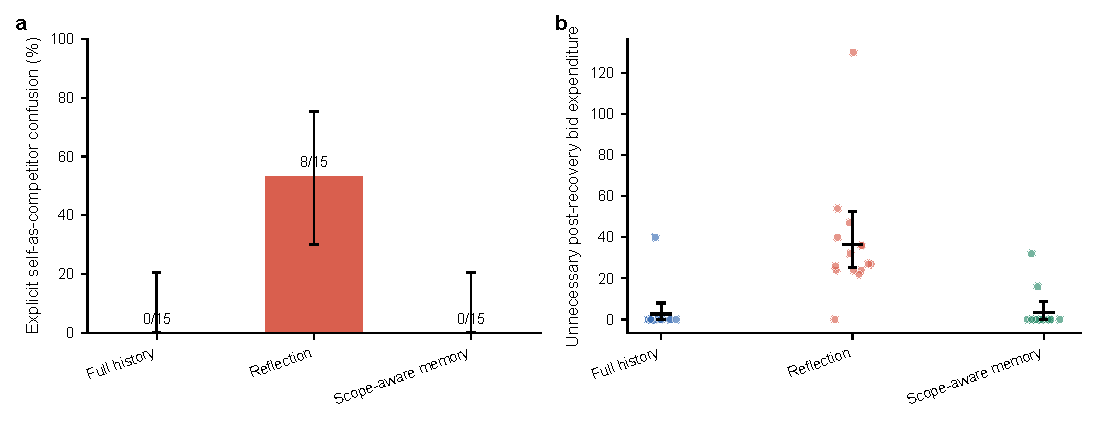
\includegraphics[width=\columnwidth]{figures/consequence_identity_confusion.pdf}
  \caption{Reflection converts the focal agent's own settlement identity into a
  competitor. \textbf{(a)} Share of auction trajectories containing an explicit
  post-event self-as-competitor statement; error bars are Wilson 95\% intervals
  over 15 trajectories. \textbf{(b)} Unnecessary post-recovery winning-bid
  expenditure relative to the sufficient bid of 50; dots are trajectories, bars
  are means with bootstrap 95\% intervals.}
  \Description{Two panels. The left panel shows Reflection at roughly 53 percent
  of auction trajectories exhibiting self-as-competitor confusion, with Full
  History and the scope-aware controller at zero. The right panel shows
  Reflection incurring much larger unnecessary bid expenditure than either
  control.}
  \label{fig:identity}
\end{figure}

\paragraph{What the consequences are, and are not.}
The other two domains show smaller but real costs. In the fishery, Reflection
remained overcautious after a named fisher returned to normal, losing a mean
4.8 harvest units in 2/5 trajectories while both controls lost none; one
trajectory generalized a single participant's overharvest to the whole group and
recorded that the others were ``self-interested maximum extractors.'' In public
goods, a single round of zero contribution by one named participant produced
post-recovery welfare loss in 3/5 Reflection trajectories (mean 8.0 units, CI
$[2.0,14.0]$), again zero for both controls. We state the negative results
plainly: no method reached the predefined extreme action zones, the fish stock
returned to and stayed at capacity, partner contributions recovered fully, and
no persona drift occurred under any method. The supported claim is that
misconsolidation imposes measurable private and welfare costs, not that it
causes ecological collapse or durable social breakdown at this horizon.

\subsection{Q3: Component Ablation}
\label{sec:ablation}

We reran the frozen held-out suite with six leave-one-section-out variants of
\egm{} (288 checkpoints, no failed trials, and no variant ever recreated its
excluded heading), and separately with a compact four-section baseline that
removes both slow sections, plus its four leave-one-out variants (240
checkpoints). Table~\ref{tab:ablation} reports the sections with a measurable
effect.

\begin{table}[t]
  \caption{Leave-one-out ablation on the frozen held-out suite (48 checkpoints
  per condition). Violation is the mean normalized distance outside the
  registered acceptable action interval. Only \textsc{action policy} shows a
  large, reliable effect, and it is behavioral rather than cognitive.}
  \label{tab:ablation}
  \centering
  \small
  \setlength{\tabcolsep}{3.0pt}
  \begin{tabular}{@{}lccc@{}}
    \toprule
    Condition & Scope $\uparrow$ & Action $\uparrow$ & Violation $\downarrow$ \\
    \midrule
    Six-section control          & 95.8 & 95.8 & 0.42\% \\
    \ \ w/o consolidated models  & 100.0 & 97.9 & 0.10\% \\
    \ \ w/o open hypotheses      & 100.0 & 97.9 & 0.21\% \\
    \ \ w/o recent episodes      & 95.8 & 87.5 & 1.46\% \\
    \ \ w/o action policy        & 95.8 & \textbf{72.9} & \textbf{4.27\%} \\
    \midrule
    Four-section baseline        & 97.9 & 97.9 & 0.10\% \\
    \ \ w/o action policy        & 100.0 & \textbf{81.3} & \textbf{3.02\%} \\
    \bottomrule
  \end{tabular}
\end{table}

\textsc{action policy} is the only component with strong necessity evidence.
Removing it leaves scope attribution untouched---indeed it slightly
\emph{raises} the probe score---while action accuracy falls to 72.9\% (11
regressions, 0 improvements, $p=0.00098$) and mean normalized violation rises
roughly tenfold. The failure is entirely on persistent world change:
persistent-change action accuracy falls from 91.7\% to 45.8\% while
recovery-case action accuracy stays at 100\%. The raw logs show both
under-response (retaining the old withdrawal after a documented supply cut) and
over-response (jumping to maximum irrigation when the registered proportional
range was 12--16). This is a belief-to-action failure, and it is the clearest
evidence in our study that \emph{correct attribution does not imply correct
behavior}---which is why Section~\ref{sec:prelim} scores both.

\textsc{recent observed episodes} shows a smaller, directionally consistent
behavioral contribution in both ablation families but remains underpowered. We
explicitly do \emph{not} claim that all six sections are independently
necessary. The four-section baseline matches the six-section method on this
suite (97.9\% scope, 97.9\% action), so the two slow sections are not
demonstrated to help here; the held-out suite contains no targeted self-state
intervention, and persona is supplied separately in every decision header, so
those two sections are weakly identified by construction. A model-assisted
claim-level forensic audit of all 576 memory snapshots was run at temperature 0
and is consistent with these tables, but manual inspection found debatable
flags, so we treat it as an exploratory diagnostic rather than a result.

\subsection{Scaling and Long-Horizon Evaluation}
\label{sec:scale}

The experiments above use short, explicit trajectories, which is what makes
their causal interventions clean but also what limits them: the phase-transition
gate of Equation~\ref{eq:cptg} is designed for horizons at which a bounded
memory becomes mandatory rather than merely convenient. We therefore additionally
evaluate the external controller across horizon length, population size, and
context pressure, using trace-replay stress suites generated deterministically
from GovSim-compatible fishing rules and Alympics-compatible water-allocation
rules with 50 and 100 rounds, 5 and 12 observed participants, matched world and
named-other persistent changes, explicit but irrelevant social distractors, and
four frozen checkpoints per trajectory. Table~\ref{tab:scale} reports the
resulting comparison across memory methods.

% TODO(paper team): insert the completed long-scale / large-scale / small-scale
% results here, then fill Table~\ref{tab:scale} and replace this placeholder
% paragraph with the analysis. Keep the same reporting discipline used above:
% report completion counts, refuse aggregates over unbalanced cells, and mark
% descriptive p-values as descriptive.

\begin{table}[t]
  \caption{Scaling evaluation across horizon length and observed population
  size. \textsc{[Placeholder --- to be completed with the frozen scale runs.]}}
  \label{tab:scale}
  \centering
  \small
  \setlength{\tabcolsep}{3.0pt}
  \begin{tabular}{@{}lccc@{}}
    \toprule
    Method & Scope $\uparrow$ & Action $\uparrow$ & Leakage $\downarrow$ \\
    \midrule
    Full History         & --- & --- & --- \\
    Reflection           & --- & --- & --- \\
    External controller  & --- & --- & --- \\
    \bottomrule
  \end{tabular}
\end{table}

\section{Limitations}
\label{sec:limitations}

Our scenarios are synthetic diagnostic vignettes inspired by GovSim and
ALYMPICS, not executions of those closed-loop benchmarks; the results
characterize the memory updater, and integrating the interventions into the
original environments remains necessary before claiming benchmark-level effects.
The attribution readout is an elicited self-report rather than direct access to
a latent belief, which is why we retain and score the persistent memory text and
the later action alongside it. Statistical power is limited: the held-out
diagnostic rests on eight scenario families and three repeats, and the
consequence experiment on three domains and five repeats, so checkpoints are
clustered and every reported $p$-value is descriptive. The consequence
experiment uses rule-based partners by design, which buys causal isolation at
the cost of not yet being a fully endogenous multi-agent society. All live runs
use a single model family, so model-dependence is untested. Several
scenario-registered action intervals encode provisional policy judgments, and at
least one scenario---a fault in the participant's own machine---is ontologically
ambiguous between \textsc{self} and \textsc{world}; the central result survives
its exclusion, but the ontology needs a precise operational definition. Finally,
the external controller is not perfect: isolated auction overbids still occurred,
and its evidence gating depends on an event parser that must be extended for
open-ended natural-language environments.

\section{Conclusion}

Social simulations increasingly rely on agents that convert an unbounded
interaction history into a bounded persistent state, and reflection is the usual
operator for that conversion. We showed that this operator can fail in a way
outcome-level evaluation does not see: the event remains legible while its
epistemic address---causal target, entity, and temporal status---silently
changes. \method{} makes that failure measurable by pairing matched trajectories
with similar visible consequences but different latent causes and auditing the
whole event $\rightarrow$ memory $\rightarrow$ attribution $\rightarrow$ action
chain. The failure is selective rather than universal: Full History usually
preserves causal distinctions, whereas free-form reflection is most brittle on
conditional and recovered evidence. It is also consequential, producing
persistent action deviation and measurable expenditure and welfare costs, most
starkly when an agent reinterprets its own settlement identity as a rival.
Gating consolidation on evidence and causal target---while keeping immediate
reversible response on a separate path---removes most of these failures at a
smaller memory footprint.

The methodological implication is the durable one. When a simulated society
behaves unexpectedly, the effect may originate in the memory updater rather than
in the personas, institutions, or interactions under study. Social-agent memory
should therefore be evaluated as a belief-update process with an auditable
address, not assumed to be benign transcript compression.

\bibliographystyle{ACM-Reference-Format}
\bibliography{references}

\end{document}
